\chapter{Deep Learning Basics}
\label{chap:deep_learning}

Deep learning has revolutionized the field of collider physics, and the performance gain observed in many algorithms used in the ATLAS experiment has substantial.
One of the most successful stories has been deep learning based algorithms for flavour tagging, covered in \Cref{sec:flavor_tagging}.
However, despite the enthusiastic integration of ML tools and techniques in HEP, the swift pace of advancements presents a unique challenge.
Researchers often find themselves in a situation where, by the time a newly developed ML tool is implemented and fully integrated into experiments, the technology has already progressed, leading to newer methodologies that render previous tools obsolete.
In addition, experimentalists in HEP favour tools with greater, robustness, and domain adaptation
The final point is relevant as most models are trained on simulated data.

This chapter provides a brief introduction to deep learning, focusing on the core concepts and techniques that are relevant to the rest of the thesis.

\section{Definition}

Deep learning is the subset of machine learning that focuses on the development and training of artificial neural networks.
These neural networks take the form of a series of composable, parametrized, and differentiable transformations that map input data to output data.
Training or optimization of the networks is done by modifying the parameters of each transformation to minimize some error metric evaluated over a dataset.
The exact form of how the error metric or loss function is calculated differentiates the various types of learning, such as supervised, unsupervised, self-supervised and reinforcement\footnote{There is often overlap between these categories}.

Initially, artificial neural networks were inspired by the structure of the brain, with many layers of interconnected artificial neurons processing information and sending signals to each other.
While individual neurons are simple, the emergent behaviour of the network can be complex.
As the field has evolved, the initial biological inspiration of neural networks has given way to more abstract, mathematical descriptions.
Today, network design is driven by inductive biases, computational efficiency, observations in training dynamics, and (above all) empirical results.
From this more practical perspective, an artificial neural network is long computational graph composed of differentiable operations arranged in layers that transform between collections of real-valued tensors.
The ``depth'' of a deep learning model often refers to the number of layers used in the network.

The primary distinction between deep learning and other parametrized curve fitting methods is simply a matter of scale.
Modern networks now contain billions of parameters, requiring large datasets, specialized hardware, and sophisticated optimization algorithms to train effectively.
As the networks have grown in size and complexity, model interpretability has become a significant challenge and an active area of research.

\section{Supervised Learning}
\label{sec:supervised_learning}

Supervised Learning is often introduced first in a pedagogical setting, as it is the simplest and most intuitive form of machine learning. While it is not limited to deep learning, it is introduced here within its context as it is arguably the most common form of training for deep models. Indeed, many other training frameworks, such as reinforcement learning, are reframed as supervised problems to facilitate training.

In supervised learning, a single data sample is a coupling of two variables $(x, y)$ and is drawn from unknown joint distribution $p_{XY}(X, Y)$.
In this setting, $x$ is the observable information about the sample, and thus the input for a model, and $y$ is some truth label, target, or desired output for a model.
The goal of supervised learning is to produce a discriminative model which approximates the mapping from inputs to outputs, $f: X \rightarrow Y$.
Discriminative models can also be probabilistic, where they model the conditional probability distribution of the target given an observation $f(x, \hat y) \approx p_Y(Y=\hat y|X=x)$.
Probabilistic models which permit sampling from this distribution can also be considered generative models, which are covered in \Cref{ch:generative_models}.

Fitting or training a supervised learning model typically requires a training set $\mathcal{D}$ containing of $N$ observations and their paired targets $\mathcal{D} = \{(x_i, y_i)\}_{i=1}^N$.
These samples are usually assumed to be independent and identically distributed (i.i.d.) from the joint\footnote{Non i.i.d. data can sometimes be used by incorporating the appropriate weights during training}.
A supervised learning algorithm $f$, probabilistic or not, is selected out of some hypothesis space $\mathcal{H}$ to minimize some measure of empirical risk $\mathcal{R}$ over the training set.
\begin{equation}
    f = \argmin_{f \in \mathcal{H}} \frac{1}{N} \sum_{i=1}^N \mathcal{R}(f, (x_i, y_i)).
\end{equation}

For now, we make no assumptions about the structure of the input or output samples except that they can be represented as tensors, or collections of tensors, of real numbers.
Common types of supervised algorithms $f$ including support vector machines, decision trees, and of course neural networks.
For a neural network $f_{\theta}$, the hypothesis space $\mathcal{H}$ is the set of all possible network architectures and network parameter values $\theta$.

\section{Network Design}

A single network layer is any function parametrized by a set of variables $\theta$ that can takes in a set of input tensors and returns a set of output tensors (both could be sets of size one).
There are very few limits on what exactly this function can be, but there are some core design principles ML engineers have to rely on when designing a network to solve a specific task.
These principles are called inductive biases~\cite{InductiveBiases1, InductiveBiases2}, and they are the assumptions made to allow a learning algorithm to favour one solution over another.
Inductive biases do not have to be explicitly defined.
For example, fitting a linear regression model explicitly assumes that the relationship between the input and output is linear, but doing so using mean squared error implicitly assumes that the relationship is corrupted by Gaussian noise with constant variance.

There exists a vast array of possible network layers, each with their own inductive biases, some as simple as affine transformations, others as complex and composite as multi-headed attention layers~\cite{Attention}.
Much of the art of deep learning is the design and composition of these layers to create a network that can solve a specific task.
One rough philosophy is that individual layers should be simple and easy to implement.
This is because neural networks are compositional, and it is the application of many of these highly parametrized layers in series that gives the network its expressive power.

As it is in physics, exploiting symmetries of the data structure is a good core principle to follow and many layers are designed with equivariance or invariance in mind.
Convolutional layers~\cite{DeepLearning} are well suited for image or otherwise grid-like data with localized features as they are somewhat equivariant to translations.
Message passing networks~\cite{NeuralMessagePassing} work well for graph data as they are equivariant to the permutation of the nodes.
GATr~\cite{GeometricAlgebraTransformer} layers are designed under the principles of Clifford algebra to operate on geometric data and are equivariant to rotations and translations.
LorentzNet~\cite{LorentzNet} operates on particle physics data and is designed to be equivariant to boosts in reference frame.
There exist many more examples of layers designed with specific data and symmetries in mind.

For deep learning, examples of inductive biases include the choice of loss function, regularization, the optimization algorithm, and even the model architecture itself.
Weight decay can be seen as an inductive bias towards simpler models, as it prioritizes solutions with small parameters.
Ideal inductive biases should improve the performance of the model primarily by aiding the optimization process.
However, too restrictive biases can limit model performance by excluding valid solutions.
Inductive biases can also be understood in terms of the bias-variance trade-off, where flexibility is traded for generalization.

\subsection{The Multi-Layer Perceptron}

The Multi-Layer Perceptron (MLP) is arguably the simplest form of a deep neural network.
It is also referred to as a dense network, fully connected network, or sometimes confusingly as a feed-forward neural network (FFN)\footnote{A term which can be used to describe any neural network without loops in the computational graph.}.
In an MLP, there is a single input and single output both of which are rank-1 tensors but can have differing numbers of features.
A minimal working example of an MLP is a series of affine transformations\footnote{Often called a linear layer, but the operation almost always includes a bias term.}, each parametrized by a weight matrix $\W$ and bias vector $\bias$, followed by a non-linear activation function $\sigma$.
The depth of the MLP is the number of intermediate representations in the computational graph between the input and output.
A minimal MLP with two hidden layers can be written as
\begin{align}
    \ba_0 &= \x, \\
    \ba_1 &= \sigma_0(\W_0 \ba_0 + \bias_0), \\
    \ba_2 &= \sigma_1(\W_1 \ba_1 + \bias_1), \\
    \ba_3 &= \sigma_2(\W_2 \ba_2 + \bias_2) = \hat{\y},
\end{align}
where $\x$ is the input, $\hat{\y}$ is the output, and $\ba_i$ are the intermediate representations (or activations) of the network.
The parameters of this network are is the full set of weights and biases from each layer, $\theta = \{W_0, \bias_0, W_1, \bias_1, W_2, \bias_2\}$.
Each layer can arbitrarily resize the input tensor based on the shapes of the weight matrix and bias vector.

Activation functions exist to introduce non-linearities in the computational graph and are applied elementwise to the tensors.
As the composition of affine transformations is itself an affine transformation, without activation functions, the entire MLP could be reparametrized as a single affine transformation, no matter its depth, greatly hindering its expressive power.
With these induced non-linearities, MLPs can approximate any continuous function between real valued tensors~\cite{ApproximationSuperpositionsSigmoidal, ApproximatingContinuousFunctions, UniversalApproximationDeep}, given enough hidden units and the right activation functions.

The activation function in the output layer is typically chosen to match the expected range of the target variable.
Historically, the sigmoid function was used as the primary activation in the hidden layers, due to its analogy with biological activation.
However, it can be shown that even the simplest function that breaks linearity is sufficient, and the ReLU~\cite{ReLU} function $\text{ReLU}(x) = \max(0, x)$ has become the popular choice for hidden layers in modern networks.
Other common choices for hidden layer activations are shown in \Cref{fig:activations}.

\begin{figure}
    \centering
    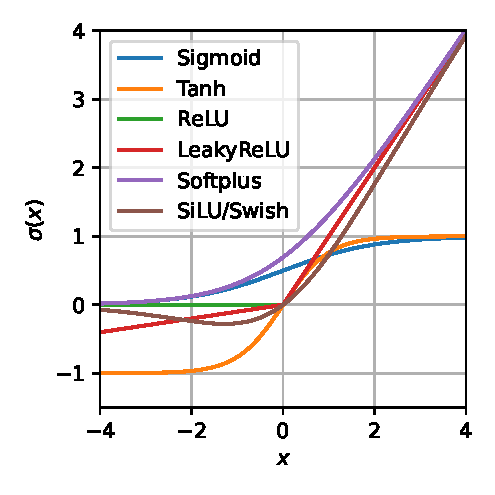
\includegraphics[width=0.4\textwidth]{Figures/transformers/activations.pdf}
    \caption{Common activation functions used in deep learning.}
    \label{fig:activations}
\end{figure}

\section{Training with Gradient Descent}

Once a network has been designed, it is typically initialized with random parameter values $\theta$.
Training or fitting a deep neural network is an optimization problem where the best parameters $\theta^*$ are those that minimize the risk, here described as a loss $\mathcal{L}$, over the training set $\mathcal{D}$.
\begin{equation}
    \theta^* = \argmin_{\theta} \frac{1}{N} \sum_{i=1}^N \mathcal{L}(\theta, x_i).
\end{equation}
For generalization, $x_i \in \mathcal{D}$ may also include the target if present.
Due to the size of the parameter space and the non-linearity of the model, the $\theta^*$ can not be found analytically.
The most common method for training deep neural networks is mini-batch stochastic gradient descent (SGD)~\cite{Perceptron} or one of its many variants.
SGD is an iterative optimization algorithm that attempts to minimize the loss over a dataset by adjusting the parameters of the model in the direction of the negative gradient of the loss calculated over a random subset of the data.
An outline of the basic training algorithm is shown in \Cref{alg:gradient_descent}.
Here $\mathcal{L}(\theta, b)$ is the average loss over a mini-batch of size $B$,
\begin{equation}
    \mathcal{L}(\theta, b) = \frac{1}{B} \sum_{i=1}^B \mathcal{L}(\theta, x_i).
\end{equation}
Both the $B$ and the $\eta$ are hyperparameters of the training algorithm.

\begin{algorithm}
    \caption{Basic training pseudocode for minibatch stochastic gradient descent.}
    \label{alg:gradient_descent}
    \begin{algorithmic}[1]
    \State \textbf{Input:} Training set $\mathcal{D}$, batch size $B$, learning rate $\eta$, stopping criterion
    \State Initialize parameters $\theta$
    \Repeat \Comment{Each loop is an \textit{epoch}}
        \State Shuffle the dataset $\mathcal{D}$
        \State Partition $\mathcal{D}$ into batches of size $B$
        \For{each batch $b$ in $\mathcal{D}$}
            \State Calculate the loss $\mathcal{L}_b(\theta)$ for the batch $b$
            \State Compute the gradient $\nabla_\theta \mathcal{L}(\theta, b)$
            \State Update parameters: $\theta \gets \theta - \eta \nabla_\theta \mathcal{L}(\theta, b)$
        \EndFor
    \Until{stopping criterion is met}
    \end{algorithmic}
\end{algorithm}

Once the entire training set has been processed, this is considered one epoch.
Training continues until some stopping criterion is met, such as a saturation of the loss.
Typically, models are trained for many epochs and the training set is shuffled between each epoch to prevent correlated updates which may hinder convergence.
Ideally we would have $B=N$, this is called batch gradient descent, but this is often infeasible due to memory constraints.
So instead we use a noisy estimate of the gradient, by using a subset of the training set and true SGD uses $B=1$.

The learning rate $\eta$ is a crucial hyperparameter of the training algorithm, however it is common to modify it during training.
Many large networks require a warm-up phase~\cite{SGDRStochasticGradient} where the learning rate is slowly increased from zero to its maximal value.
Without this step, large models like transformers are prone to diverging early in training.
The learning rate is also typically decayed towards the end of training helping the network converge to a local minimum, avoiding oscillation, and improving the learning of complex patterns~\cite{HowDoesLearning}.
Sometimes these phases are repeated, cycling the learning rate up and down again and again~\cite{CyclicalLearningRates}, and sometimes they are performed only once~\cite{SuperConvergenceVeryFast}, ending the training after the first cycle.

There exist many extensions to this basic algorithm that attempt to improve robustness and convergence.
One common method is the accumulation of a moving average of the gradients, analogous to momentum in physics~\cite{Momentum}.
This assists in traversing regions of the parameter space where curvature is higher in one direction than another.
Another common method is the use of adaptive learning rates, where the per parameter learning rate is adjusted based on the fluctuations in the gradient~\cite{Adagrad, RMSProp}.
\Cref{alg:adam} shows the update rule for one of the most common variants, the Adam optimizer~\cite{Adam}, which combines both momentum and adaptive learning rates.
It introduces two hyperparameters $\beta_1$ and $\beta_2$ which control the exponential decay rates of the moving averages.

\begin{algorithm}
\caption{The Adam optimizer, where $\mathcal{L}(\theta, b)$ is the loss calculated over a mini-batch, $\eta$, $\beta_1$, $\beta_2$ are hyperparameters, $t$ is the current iteration and $\epsilon$ is a small constant to prevent division by zero.}
\label{alg:adam}
\begin{algorithmic}[1]
\State $\mathbf{m} \gets 0$ \Comment{Initialize first moment vector}
\State $\mathbf{s} \gets 0$ \Comment{Initialize second moment vector}
\For{each mini-batch $b$}
    \State $\mathbf{g} \gets \nabla_\theta \mathcal{L}(\theta, b)$ \Comment{Compute gradients}
    \State $\mathbf{m} \gets \beta_1 \mathbf{m} + (1 - \beta_1) \mathbf{g}$ \Comment{Update biased first moment estimate}
    \State $\mathbf{s} \gets \beta_2 \mathbf{s} + (1 - \beta_2) \mathbf{g} \otimes \mathbf{g}$ \Comment{Update biased second moment estimate}
    \State $\hat{\mathbf{m}} \gets \frac{\mathbf{m}}{1 - \beta_1^t}$ \Comment{Correct bias in first moment}
    \State $\hat{\mathbf{s}} \gets \frac{\mathbf{s}}{1 - \beta_2^t}$ \Comment{Correct bias in second moment}
    \State $\theta \gets \theta - \eta \frac{\hat{\mathbf{m}}}{\sqrt{\hat{\mathbf{s}} + \epsilon}}$ \Comment{Update parameters}
\EndFor
\end{algorithmic}
\end{algorithm}

\subsection{Normalization}

Training via gradient descent requires the gradient with respect to every parameter in the model.
This leads to a balancing problem with the vanishing and exploding gradient problems manifesting as the gradients become too small or too large to be useful for training.
This is especially problematic in deep networks, where the gradients must be propagated through many layers, requiring the repeated application of the chain rule.
As the scale of the gradients are linked to the scale of the activations in each layer, it is good practice to ensure the activations remain within a reasonable range during training.
It is common to target activations with a mean of zero and unit variance through the inclusion of normalization layers.

In addition to stabilizing gradients, normalization layers assist in the expressivity of the networks.
Most activation non-linearities occur near zero, \Cref{fig:activations}.
Oversaturating these functions with large positive or negative values ensure that the layer either becomes linear or constant, depending on the function.
In both cases, the layer can no longer approximate non-linear transformations.

Normalization starts with the input data itself, which can be seen as a preprocessing step or as the first layer of the network.
This is typically performed using the statistics of the training set.
Variables with long tails are also transformed to have a more Gaussian distribution.
This can be done by taking the logaritm of variables with large dynamic ranges, or by using more advanced techniques like a quantile transformation.
Within the network itself, normalization layers $L_{\text{norm}}$ are interleaved between others.
Methods such as batch normalization~\cite{BatchNorm} or layer normalization~\cite{LayerNorm} are widely used and both have been shown to be greatly effective, with the latter seen as essential for transformer neural networks~\cite{Attention}.

Another feature used to stabilize training is the manual clipping of the gradients before applying the parameter update.
This can be done based on some maximal value, but is more commonly done by scaling the gradient such that their combined norm does not exceed some threshold~\cite{WhyGradientClipping}.

\subsection{Residual Connections}

Residual connections are another simple and effective technique for training deep networks.
Here the learnable transformation of the layer is added to the input, rather than replacing it,
\begin{equation}
    \ba_{i+1} = \ba_i + l(\ba_i),
\end{equation}
where $l$ is the transformation of the layer.
A single operation of this form is called a residual block.
Residual connections have been shown to improve the training of very deep networks, as they allow the gradient to flow directly through the network, bypassing the squashing or exploding effects of the intermediate layers.
Residual connections are a key component of almost all modern architectures from convolutional neural networks~\cite{ResNet} to transformers~\cite{Attention}.
The residual connection is usually additive, but other operations exist, for example UNets~\cite{UNet} use concatenation.
If the input and output of the layer have different dimensions, the residual path can be adjusted by a minimal transformation, in a convolutional network this is typically a $1 \times 1$ convolution.

The addition of two signal paths means that $a_{i+1}$ will have a larger variance than $a_i$.
This can cause a deeper network to become unstable, especially in the early stages of training.
One method to circumvent this is the inclusion of a normalization layer after the residual block, as was done in the original transformer architecture~\cite{Attention}, which is referred to as post-normalization.
However, this was shown to be detrimental in very deep networks and recent methods use pre-normalization~\cite{PreLN} (PreNorm), where the input to the learnable layer is normalized.
With a PreNorm residual block one can prevent an exploding variance problem by scaling the residual path by a small constant, such as $\frac{1}{\sqrt{2}}$~\cite{StyleGAN2}.
Recent methods allow this constant to be trainable with some set it to zero at the beginning of training such that the block behaves like an identity function~\cite{ReZero, SkipInit, Fixup}.
This was extended to the LayerScale method~\cite{GoingDeeper}, where a fully learnable tensor $\mathbf{L}_\text{scale}$ matching the output shape of the layer is used to scale the residual path.
Initialized to zero, the network will learn the optimal scaling during training.

A PreNorm residual block with LayerScale follows,
\begin{equation}
    \ba_{i+1} = \ba_i + \mathbf{L}_\text{scale} \otimes f( L_{\text{norm}}(\ba_i) ),
\end{equation}
where $\otimes$ is elementwise multiplication.
Such a layer structure can be applied in many types of networks, from MLPs~\cite{InvertedBottleneck} to transformers~\cite{GoingDeeper}.

\section{Generalization}

Generalization in the context of ML refers to the ability of a model to perform well on new, unseen data.
This is in most cases the primary goal of training such a model.
As neural networks are highly flexible, it is possible that they can ``memorize'' the training set, achieving a very low loss during training, but not matching that performance on new data.
This phenomenon is called overfitting, and it is a common problem in deep learning.

Overfitting may be detected during training through cross-validation.
The most simple case of this is to split the available data into a training set and a validation set.
Gradient descent is performed on the training set, but the loss is also calculated over the validation set at regular intervals.
The difference in performance between the training and validation set is a good indicator of overfitting.
Often the model chosen for future applications is the one that performs best on the validation set.

There are many methods to combat or reduce overfitting.
Regularization methods are techniques that affect the training process.
Weight decay includes extra terms in the loss function that impose a penalty based on the magnitude of the parameters in the network, pushing it towards simpler solutions.
Dropout~\cite{Dropout} is a technique where a random subset of the activations in the network are set to zero during training, effectively training an ensemble of models.
Alternatively, dropout simply injects noise into the network, which can help prevent overfitting.
Drop-path and stochastic depth~\cite{DeepNetworksStochastic} is an extension of dropout where entire residual layers are removed from the network during training.
Data augmentation can also help by artificially expanding the training dataset.
Confusingly, increasing the size of the network can also help prevent overfitting.
This is known as the double descent phenomenon~\cite{UnderstandingDoubleDescent}, whereas the effective model capacity grows, more solutions become accessible, and the model becomes a self ensemble.

Domain shift is a problem which is similar to overfitting, but occurs when the underlying distribution of the training and test datasets differ.
This is a significant issue in fields HEP, where models are trained on simulated samples, in order to have access to ground truth labels, but must be applied to real data.
Domain adaptation~\cite{UnsupervisedDomainAdaptation} and adversarial training~\cite{EnhancingGeneralizationHigh} are methods to address this.

Finally, unwanted biases in the training set can lead to skewed predictions.
The distribution of the target variable in supervised settings acts as a prior for the model, and if this distribution is not representative of the population, the model will make biased predictions.
Reweighting or resampling the training set can help mitigate this.
